\documentclass{article}
\usepackage{scimisc-cv}
\usepackage{hyperref}
\usepackage{fancyhdr}
\usepackage{graphicx}
\usepackage{xcolor}
\usepackage[export]{adjustbox}
\title{ Mikhail Solovyanov CV for Electronic Positions}
\author{Mikhail Solovyanov}
\date{\today}
 
%% These are custom commands defined in scimisc-cv.sty
\cvname{Mikhail Solovyanov}
\cvpersonalinfo{
27 years old \cvinfosep
Yerevan, Armenia \cvinfosep
+374-44-190-197 \cvinfosep
mikhail.solovyanov@gmail.com \cvinfosep
\href{https://www.linkedin.com/in/mikhail-solovyanov-b4a32b217/}{linkedin} \cvinfosep
\href{https://github.com/mikprin}{github}
}
 
%\rhead{\begin{picture}(0,0) \put(0,0){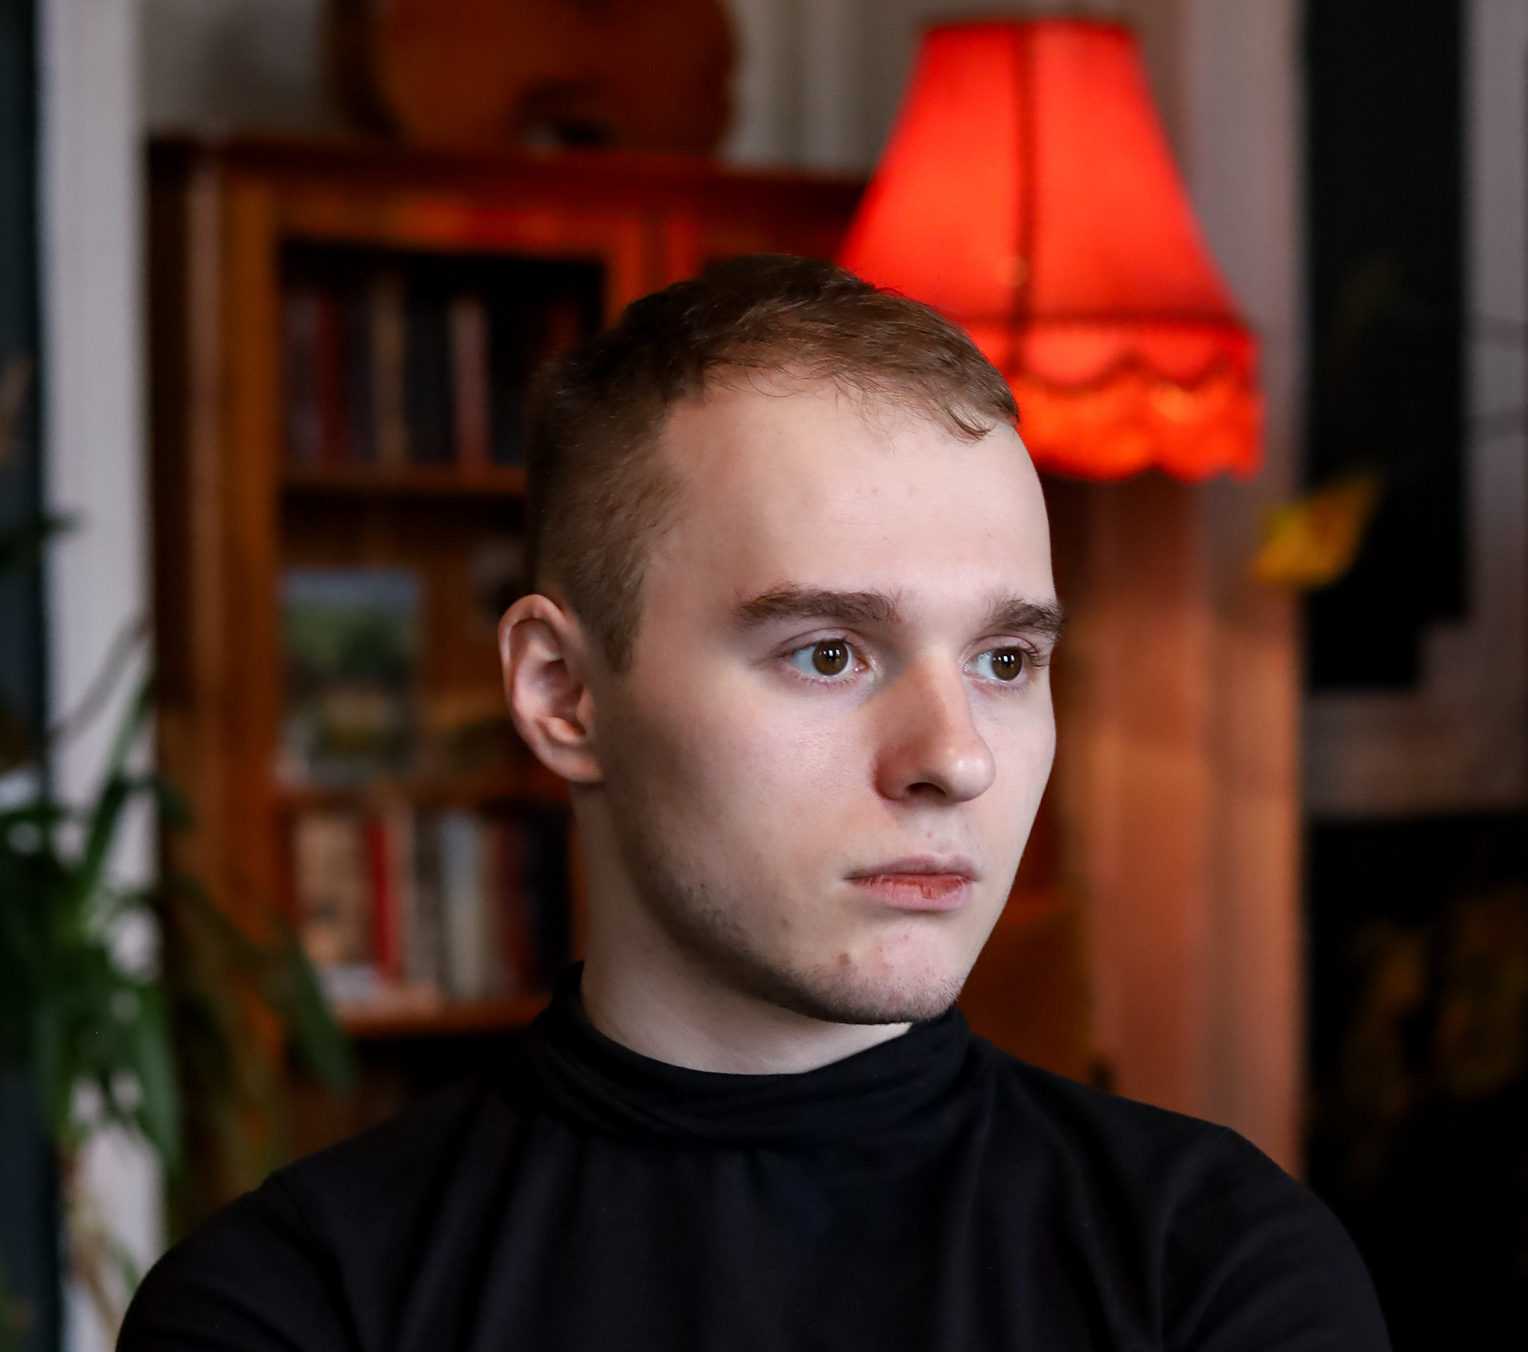
\includegraphics[width=1cm]{picture.jpg}} \end{picture}}

\begin{document}

% \maketitle %% This is LaTeX's default title constructed from \title,\author,\date
 
\makecvtitle %% This is a custom command constructing the CV title from \cvname, \cvpersonalinfo
%\smash{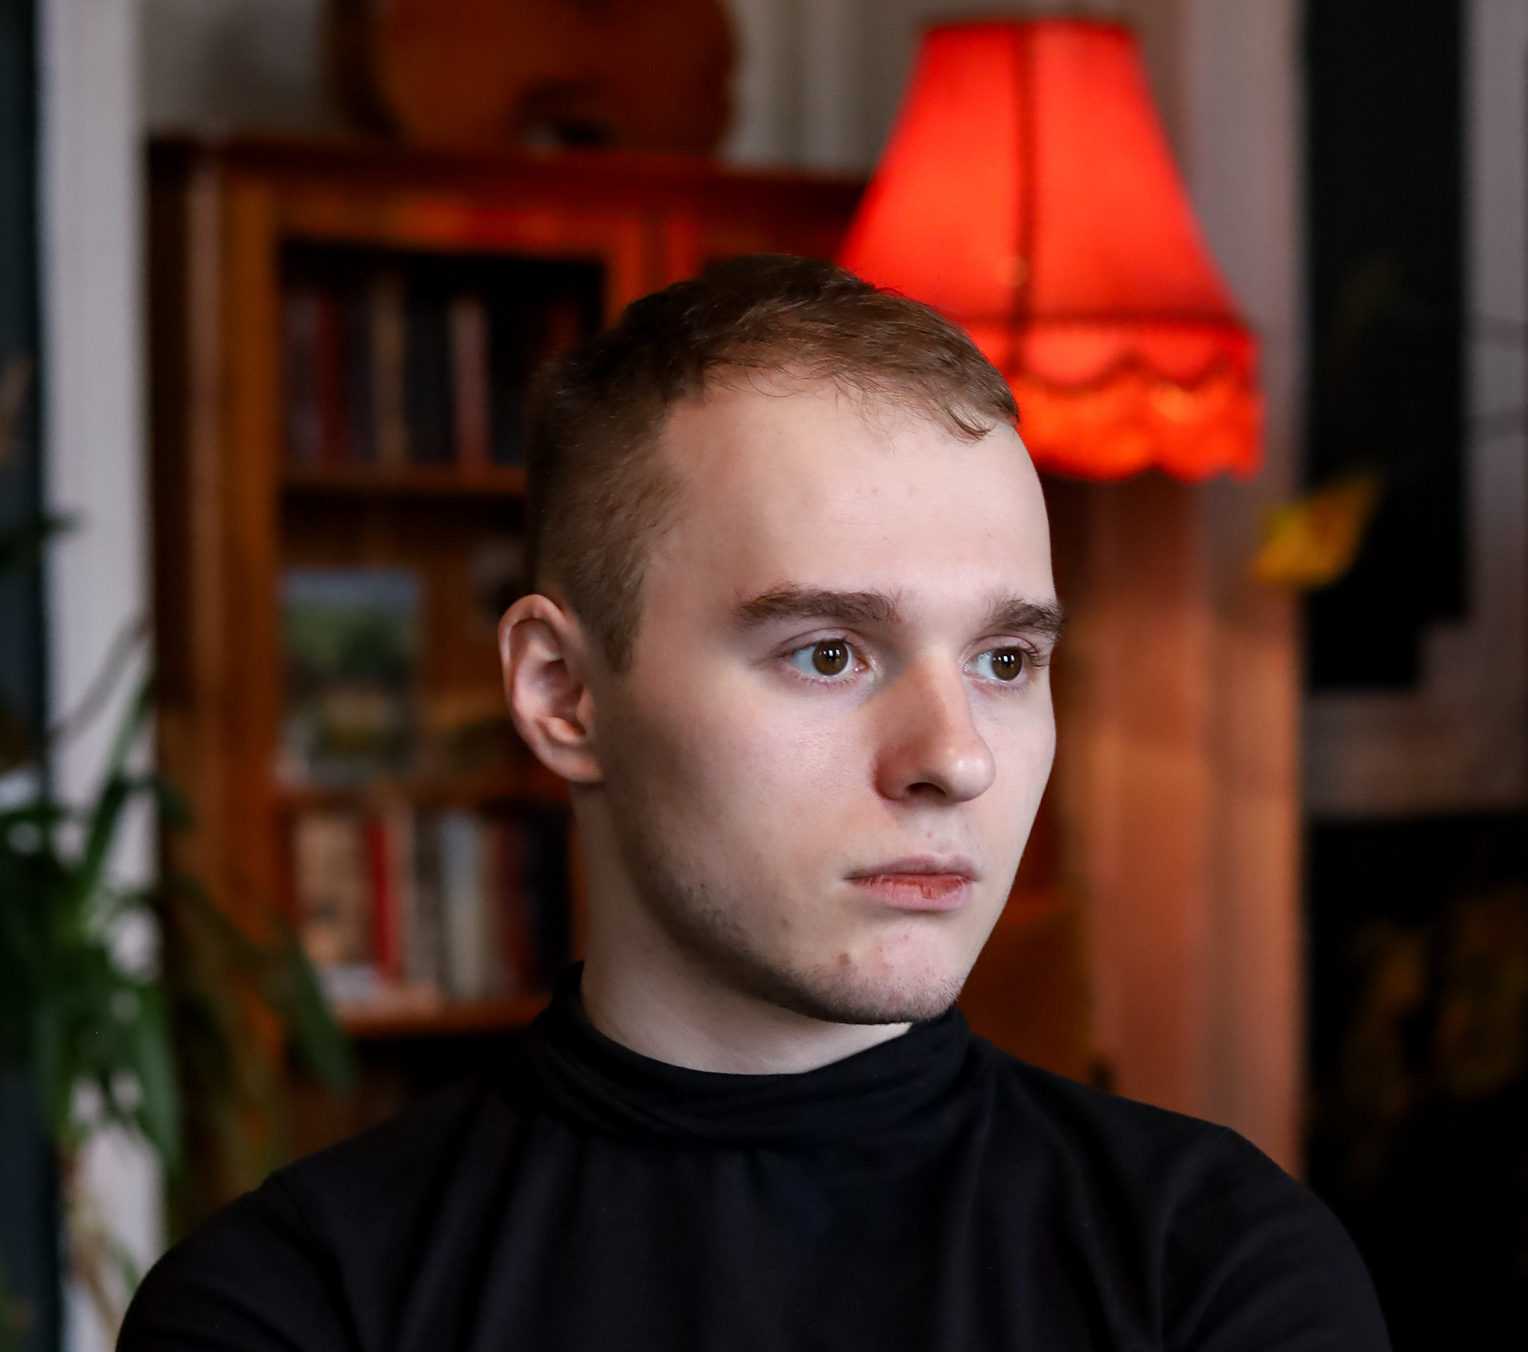
\includegraphics[width=3cm]{picture.jpg}}
%\raisebox{-.5\totalheight}[0pt][.5\totalheight]{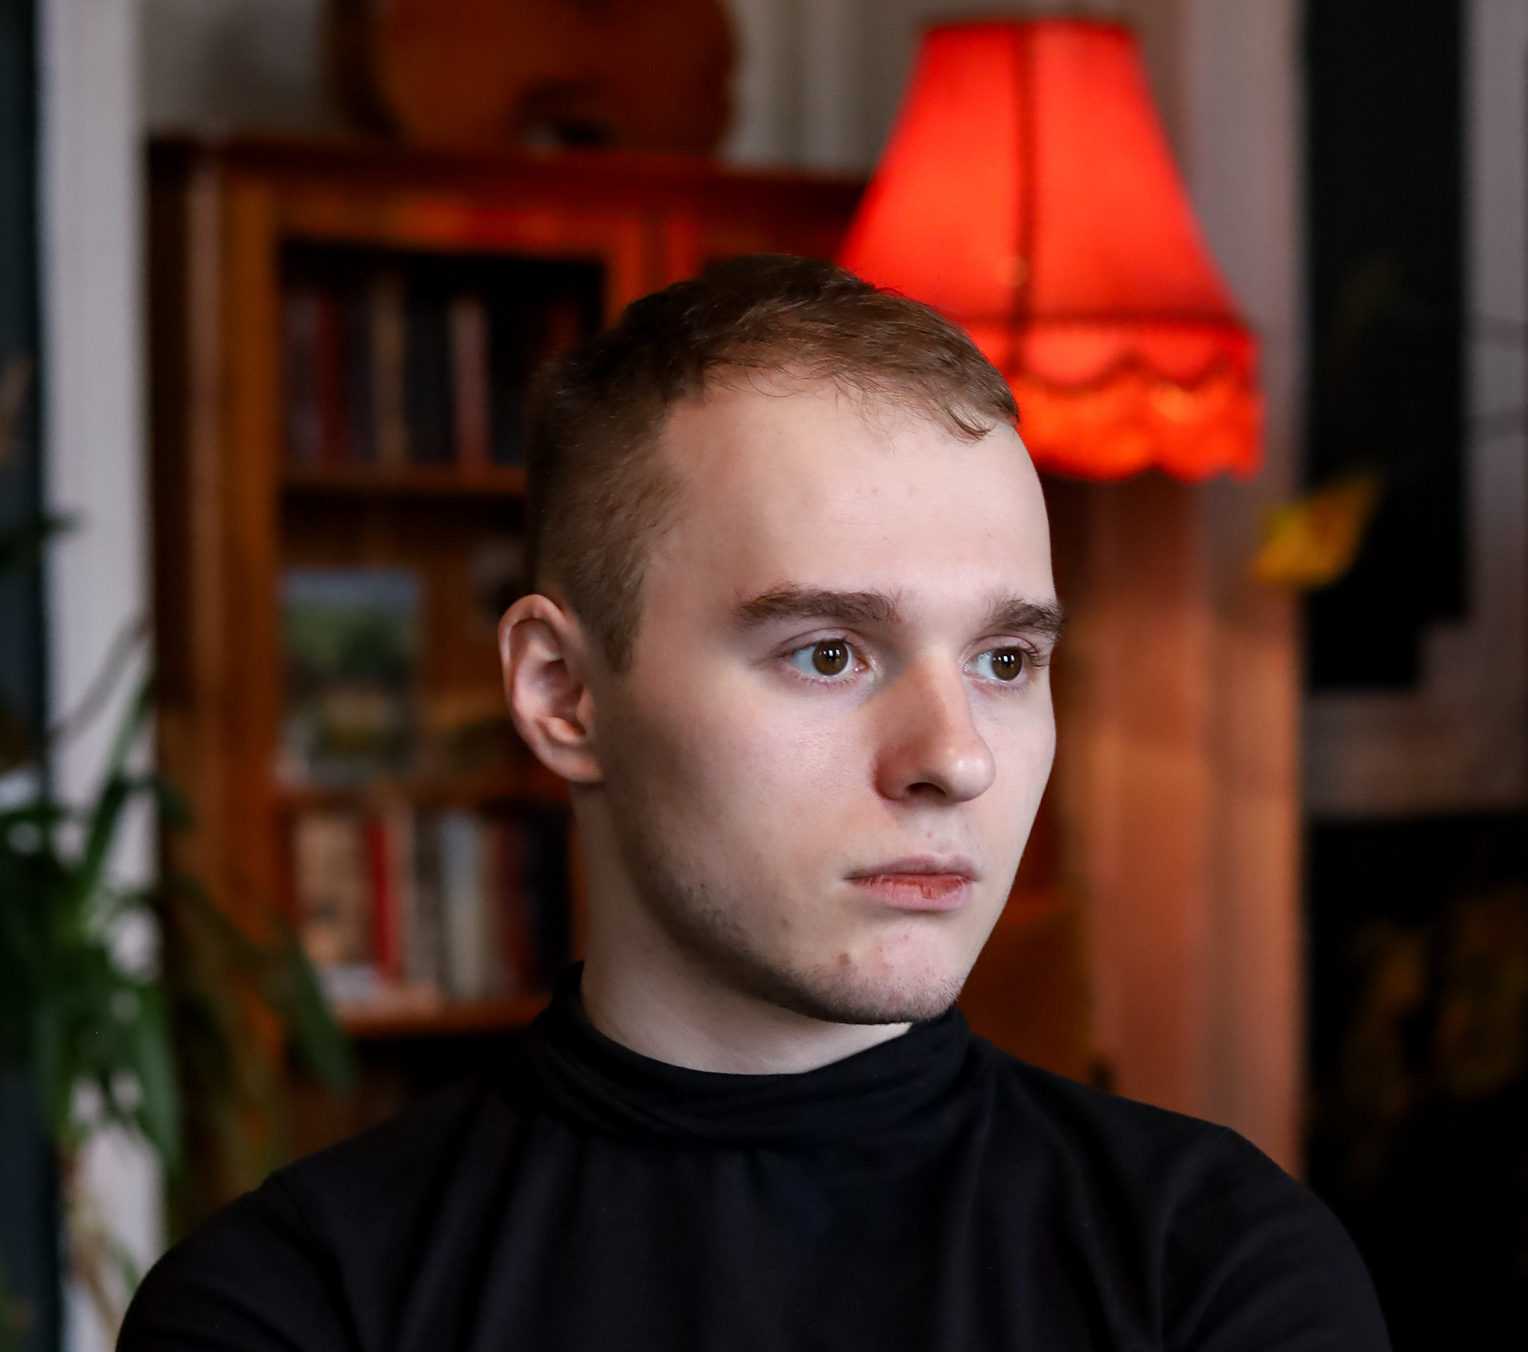
\includegraphics[width=10cm,height=10cm]{picture.jpg}}

% \section{Summary}
% \begin{minipage}{0.7\textwidth}
%    \begin{itemize}
%       \item Interdisciplinary engineer,  with skills and experience in programming, electronics, machine learning, OS and computer networks.
%       \item Led development of a project resulting in a patent.
%       \item Self-motivated, problem-solving and collaborative employee with notable communication and management skills.
%       \item Have no stress digging in interdisciplinary fields and learning new subjects on the fly.
%       \end{itemize}
%    \end{minipage}%
%    \hfill
%    \begin{minipage}{0.3\textwidth}
%       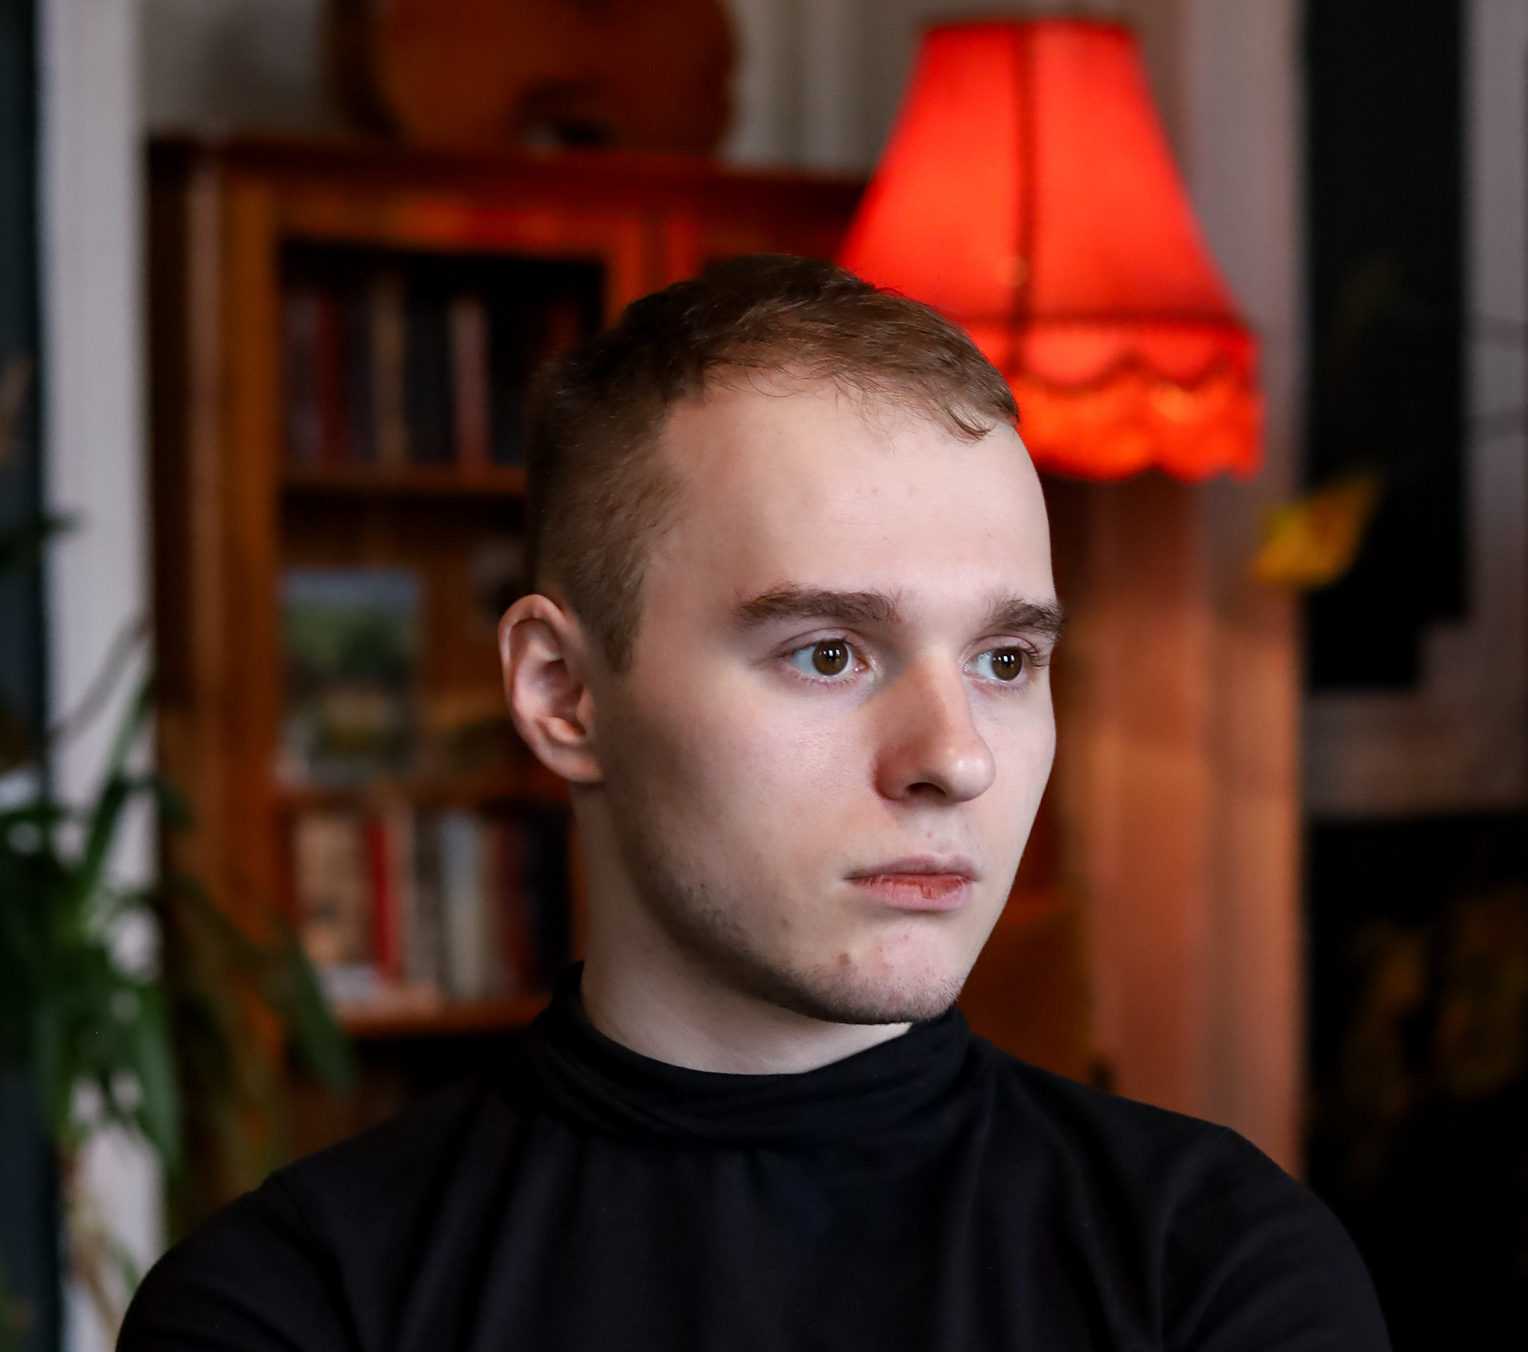
\includegraphics[width=3.5cm,right]{picture.jpg}
% \end{minipage}%


% BEGIN OF RESUME

% \section{Technical Skills}
 
% \begin{itemize}

%    \item \textbf{Software engineering:} General experience of collaborative functional and object-oriented programming. Working with data and data analysis. Data visualization. Basics of web development and backend. Digital signal processing. Embedded programming. API and service architecture.
%    \item \textbf{Networks and Computer engineering and administration:} Linux proficiency, comfortable working in various Linux environments and containers as well as Windows. Cluster management. Network administration. Network security.
%    \item \textbf{Computational and Machine Learning, computer vision:} Applied machine learning algorithms. General knowledge in ML framework programming. General knowledge of machine learning methods. Optimization algorithms and basic CV algorithms.
%    \item \textbf{Electronics design:} Analog and mixed IC electronics Design. Signals and systems, control design. Simulation and verification automation. Processor architecture understanding. FPGA programming. PCB design and microcontrollers programming, RF, IOT stack.
%    \item \textbf{Communication:} Interdisciplinary communication, engineering management, project management, presentation and explanation skills.
% \end{itemize}

\section{Software and Hardware Skills}

\begin{itemize}
   \item \textbf{DevOps and OS:} Docker, Kubernetes, Ansible, concourse, redis, Skaffold, Linux (Centos,Debian based systems, Arch), GIT, filesystems, github Actions.
   \item \textbf{High level languages:} Python, bash, SQL, MATLAB, Simulink, SimScape, HTML, Verilog, VerilogA, gnuradio.
   \item \textbf{Frameworks:} pandas, FastApi, numpy, scipy, celery, PyTorch, sklearn, threading, matplotlib, Qt, SQLAlchemy, AirFlow, Django, Flask, Prefect, polars.
   \item \textbf{System level programming languages:} C, Rust. Including FreeRTOS and register level programming.
   \item \textbf{Electronics:} Development and automation of IC design.
\end{itemize}

\section{work Experience and Research}

\cvsubsection{ \href{https://bostongene.com/}{BostonGene}, Software engineer}[October 2022 to present]
% [Data engineer][]
   \begin{itemize}
      \item Developed custom mutation database query engine using Python. This engine allowed analitics to manage 1000s of biomarkers using natural language. This project is the core or Bostongene clinical pipeline data analysis.
      \item Developed and integrated granular container based ML-ops service for bioinformatics team models. Improving ML model integration time by 50\%.
      \item Integrated and supported described services in the dynamic k8s cluster infrastructure. Also using scaffold and helm. Concourse CI/CD pipelines for them.
    \end{itemize}

\cvsubsection{ \href{https://en.wikipedia.org/wiki/Synopsys}{Synopsys}, Senior R\&D engineer}[March 2022 to October 2022]
% [][]
   \begin{itemize}
      \item Created and integrated flow for prototyping and testing team's software solutions on custom client hardware using Xilinx Zynq FPGA boards.
      \item This work led to successful presentation of "mission mode" testing solution for Qualcomm processors on International Test Safety Conference in 2022. Project was finished on time and under budget.
   \end{itemize}  

\cvsubsection{ \href{http://twin3d.pro}{Twin3d}, Leading engineer}[January 2021 to Feb 2022]
% [][January 2021 to Feb 2022]
\begin{itemize}
   \item Designed from scratch and built software, infrastructure and electrical system to trigger, access and store data for 240 DSLR cameras. This biggest rig in Russia was made for making top edge 3D photorealistic models of people and animals for VFX, games, cinema etc.
   \item Hired and managed team of 2 programmers and 2 mechanical engineers for making scanners upgrades.
   \item Built and maintained company IT infrastructure including servers and pipelines for ML-based 3D reconstruction pipelines. All of the above still creates value for the company.
\end{itemize}

\cvsubsection{\href{https://mipt.ru/english/}{MIPT Neurocomputing systems lab}, Engineer}[September 2017 to September 2021]
% [][September 2017 to September 2021]
\begin{itemize}
\item Responsible for development of a prototype of a memory  compiler for new FRAM or ReRAM memory (Python and bash).
\item Used machine learning methods to evaluate parasitics in prototype IC chips and measuring probes.
\end{itemize}

\cvsubsection{\href{http://uvl.io/ }{UVL Robotics}, Electronic engineer / DevOps}[Feb 2020 to Dec 2020]
% [Electronic engineer / DevOps][Feb 2020 to Dec 2020]
\begin{itemize}
\item Created and maintained Linux distribution with ML-tools for shipping AI powered logistic quadcopter drones based on Nvidia Jetson Xavier board.
\item Responsible for development and programming of a PCB motherboard for mentioned drones.
\end{itemize}

\section{Education}
 
\begin{itemize}
\item Masters, applied physics and math, Moscow Institute of Physics and Technology (MIPT) department of quantum and physical electronics, 2019-2021
\item BS, Bachelor of applied physics and math, Moscow Institute of Physics and Technology (MIPT) department of quantum and physical electronics, 2015-2019.
\end{itemize}
 
\section{Awards and other}
 
\begin{itemize}
\item \href{https://microelectronica.pro/}{International forum microelectronics 2019}. Thesis: "Developing high energy efficient FRAM memory in neurocomputing application".
\item \href{https://conf62.mipt.ru/}{The 62th MIPT Scientific Conference.}. Thesis "Compiler for high energy efficient FRAM memory in neurocomputing application"
\item \href{https://mipt.ru/science/5top100/education/courseproposal/%D0%A4%D0%AD%D0%A4%D0%9C.pdf}{The 63th MIPT Scientific Conference.}. Thesis: "Development of SMU IC for testing energy efficient memories"
\item Have a \href{https://www.youtube.com/channel/UCAjmXQnYQjWoVHx6NIo24CQ}{YouTube Channel} about electronics and software.
\item Mentoring and teaching experience in MIPT.
\end{itemize}
 
%\section{Publications}
%Still yet to come %
 
\section{Other Skills}
\begin{description}[widest=Langauges]
\item[Languages] English: professional proficiency.  Russian: native.
\item[Hobbies] Making electronics. Competition level dancer (WCS, Hustle), making educational \href{https://www.youtube.com/channel/UCAjmXQnYQjWoVHx6NIo24CQ}{content} on youtube.
\end{description}
\end{document}